% Created by tikzDevice version 0.11 on 2019-01-03 16:01:30
% !TEX encoding = UTF-8 Unicode
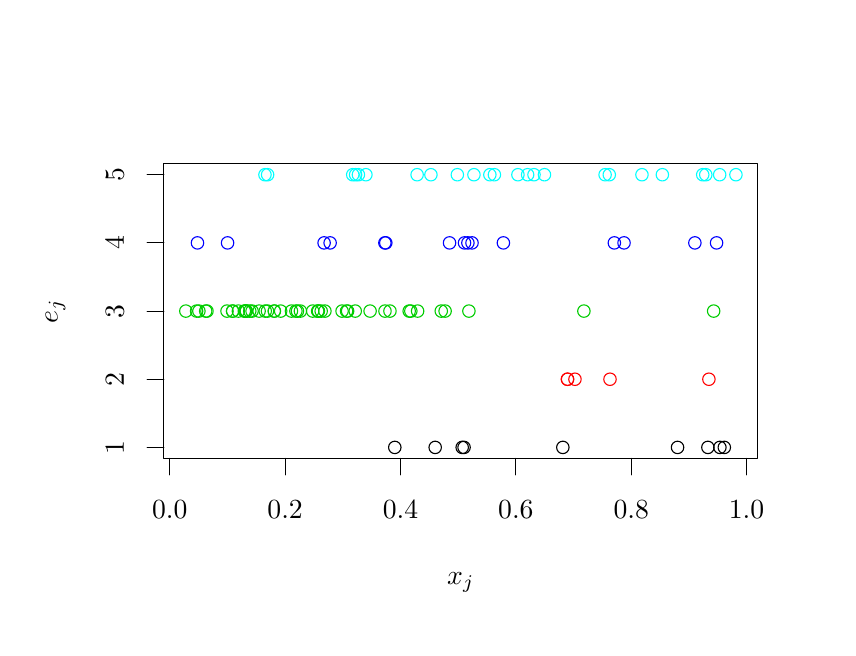
\begin{tikzpicture}[x=1pt,y=1pt]
\definecolor{fillColor}{RGB}{255,255,255}
\path[use as bounding box,fill=fillColor,fill opacity=0.00] (0,0) rectangle (289.08,216.81);
\begin{scope}
\path[clip] ( 49.20, 61.20) rectangle (263.88,167.61);
\definecolor{drawColor}{RGB}{0,0,255}

\path[draw=drawColor,line width= 0.4pt,line join=round,line cap=round] (107.11,139.04) circle (  2.25);
\definecolor{drawColor}{RGB}{0,205,0}

\path[draw=drawColor,line width= 0.4pt,line join=round,line cap=round] ( 96.93,114.40) circle (  2.25);
\definecolor{drawColor}{RGB}{0,0,255}

\path[draw=drawColor,line width= 0.4pt,line join=round,line cap=round] (159.07,139.04) circle (  2.25);
\definecolor{drawColor}{RGB}{0,205,0}

\path[draw=drawColor,line width= 0.4pt,line join=round,line cap=round] (107.41,114.40) circle (  2.25);

\path[draw=drawColor,line width= 0.4pt,line join=round,line cap=round] ( 89.12,114.40) circle (  2.25);

\path[draw=drawColor,line width= 0.4pt,line join=round,line cap=round] (159.44,114.40) circle (  2.25);
\definecolor{drawColor}{RGB}{0,255,255}

\path[draw=drawColor,line width= 0.4pt,line join=round,line cap=round] (168.65,163.67) circle (  2.25);
\definecolor{drawColor}{RGB}{0,205,0}

\path[draw=drawColor,line width= 0.4pt,line join=round,line cap=round] ( 78.28,114.40) circle (  2.25);

\path[draw=drawColor,line width= 0.4pt,line join=round,line cap=round] (104.79,114.40) circle (  2.25);

\path[draw=drawColor,line width= 0.4pt,line join=round,line cap=round] (200.99,114.40) circle (  2.25);
\definecolor{drawColor}{RGB}{0,0,0}

\path[draw=drawColor,line width= 0.4pt,line join=round,line cap=round] (251.73, 65.14) circle (  2.25);
\definecolor{drawColor}{RGB}{0,0,255}

\path[draw=drawColor,line width= 0.4pt,line join=round,line cap=round] ( 72.23,139.04) circle (  2.25);
\definecolor{drawColor}{RGB}{255,0,0}

\path[draw=drawColor,line width= 0.4pt,line join=round,line cap=round] (210.42, 89.77) circle (  2.25);
\definecolor{drawColor}{RGB}{0,0,255}

\path[draw=drawColor,line width= 0.4pt,line join=round,line cap=round] (248.93,139.04) circle (  2.25);
\definecolor{drawColor}{RGB}{0,255,255}

\path[draw=drawColor,line width= 0.4pt,line join=round,line cap=round] (221.97,163.67) circle (  2.25);
\definecolor{drawColor}{RGB}{0,205,0}

\path[draw=drawColor,line width= 0.4pt,line join=round,line cap=round] (115.61,114.40) circle (  2.25);
\definecolor{drawColor}{RGB}{0,255,255}

\path[draw=drawColor,line width= 0.4pt,line join=round,line cap=round] (186.74,163.67) circle (  2.25);

\path[draw=drawColor,line width= 0.4pt,line join=round,line cap=round] (250.05,163.67) circle (  2.25);
\definecolor{drawColor}{RGB}{0,0,0}

\path[draw=drawColor,line width= 0.4pt,line join=round,line cap=round] (250.13, 65.14) circle (  2.25);
\definecolor{drawColor}{RGB}{0,255,255}

\path[draw=drawColor,line width= 0.4pt,line join=round,line cap=round] (122.22,163.67) circle (  2.25);
\definecolor{drawColor}{RGB}{0,205,0}

\path[draw=drawColor,line width= 0.4pt,line join=round,line cap=round] (106.06,114.40) circle (  2.25);

\path[draw=drawColor,line width= 0.4pt,line join=round,line cap=round] ( 85.84,114.40) circle (  2.25);
\definecolor{drawColor}{RGB}{0,255,255}

\path[draw=drawColor,line width= 0.4pt,line join=round,line cap=round] (118.50,163.67) circle (  2.25);
\definecolor{drawColor}{RGB}{0,0,0}

\path[draw=drawColor,line width= 0.4pt,line join=round,line cap=round] (157.68, 65.14) circle (  2.25);
\definecolor{drawColor}{RGB}{0,255,255}

\path[draw=drawColor,line width= 0.4pt,line join=round,line cap=round] (243.93,163.67) circle (  2.25);
\definecolor{drawColor}{RGB}{0,0,255}

\path[draw=drawColor,line width= 0.4pt,line join=round,line cap=round] (157.85,139.04) circle (  2.25);
\definecolor{drawColor}{RGB}{0,205,0}

\path[draw=drawColor,line width= 0.4pt,line join=round,line cap=round] (105.05,114.40) circle (  2.25);

\path[draw=drawColor,line width= 0.4pt,line join=round,line cap=round] ( 61.04,114.40) circle (  2.25);

\path[draw=drawColor,line width= 0.4pt,line join=round,line cap=round] (138.45,114.40) circle (  2.25);
\definecolor{drawColor}{RGB}{0,255,255}

\path[draw=drawColor,line width= 0.4pt,line join=round,line cap=round] (229.34,163.67) circle (  2.25);
\definecolor{drawColor}{RGB}{0,205,0}

\path[draw=drawColor,line width= 0.4pt,line join=round,line cap=round] (123.73,114.40) circle (  2.25);

\path[draw=drawColor,line width= 0.4pt,line join=round,line cap=round] ( 78.75,114.40) circle (  2.25);
\definecolor{drawColor}{RGB}{0,0,255}

\path[draw=drawColor,line width= 0.4pt,line join=round,line cap=round] (129.41,139.04) circle (  2.25);
\definecolor{drawColor}{RGB}{0,255,255}

\path[draw=drawColor,line width= 0.4pt,line join=round,line cap=round] (182.96,163.67) circle (  2.25);
\definecolor{drawColor}{RGB}{0,0,0}

\path[draw=drawColor,line width= 0.4pt,line join=round,line cap=round] (132.66, 65.14) circle (  2.25);
\definecolor{drawColor}{RGB}{255,0,0}

\path[draw=drawColor,line width= 0.4pt,line join=round,line cap=round] (195.09, 89.77) circle (  2.25);

\path[draw=drawColor,line width= 0.4pt,line join=round,line cap=round] (195.04, 89.77) circle (  2.25);
\definecolor{drawColor}{RGB}{0,255,255}

\path[draw=drawColor,line width= 0.4pt,line join=round,line cap=round] (167.01,163.67) circle (  2.25);
\definecolor{drawColor}{RGB}{0,205,0}

\path[draw=drawColor,line width= 0.4pt,line join=round,line cap=round] (140.90,114.40) circle (  2.25);
\definecolor{drawColor}{RGB}{0,255,255}

\path[draw=drawColor,line width= 0.4pt,line join=round,line cap=round] (145.71,163.67) circle (  2.25);
\definecolor{drawColor}{RGB}{0,205,0}

\path[draw=drawColor,line width= 0.4pt,line join=round,line cap=round] (115.23,114.40) circle (  2.25);
\definecolor{drawColor}{RGB}{0,0,255}

\path[draw=drawColor,line width= 0.4pt,line join=round,line cap=round] (171.90,139.04) circle (  2.25);

\path[draw=drawColor,line width= 0.4pt,line join=round,line cap=round] (241.09,139.04) circle (  2.25);
\definecolor{drawColor}{RGB}{0,205,0}

\path[draw=drawColor,line width= 0.4pt,line join=round,line cap=round] ( 81.08,114.40) circle (  2.25);

\path[draw=drawColor,line width= 0.4pt,line join=round,line cap=round] (137.86,114.40) circle (  2.25);

\path[draw=drawColor,line width= 0.4pt,line join=round,line cap=round] ( 95.32,114.40) circle (  2.25);
\definecolor{drawColor}{RGB}{0,255,255}

\path[draw=drawColor,line width= 0.4pt,line join=round,line cap=round] (140.72,163.67) circle (  2.25);
\definecolor{drawColor}{RGB}{0,205,0}

\path[draw=drawColor,line width= 0.4pt,line join=round,line cap=round] ( 79.01,114.40) circle (  2.25);
\definecolor{drawColor}{RGB}{0,0,0}

\path[draw=drawColor,line width= 0.4pt,line join=round,line cap=round] (147.25, 65.14) circle (  2.25);
\definecolor{drawColor}{RGB}{0,205,0}

\path[draw=drawColor,line width= 0.4pt,line join=round,line cap=round] (247.88,114.40) circle (  2.25);
\definecolor{drawColor}{RGB}{0,255,255}

\path[draw=drawColor,line width= 0.4pt,line join=round,line cap=round] (210.16,163.67) circle (  2.25);
\definecolor{drawColor}{RGB}{0,0,0}

\path[draw=drawColor,line width= 0.4pt,line join=round,line cap=round] (245.79, 65.14) circle (  2.25);
\definecolor{drawColor}{RGB}{0,205,0}

\path[draw=drawColor,line width= 0.4pt,line join=round,line cap=round] (149.45,114.40) circle (  2.25);
\definecolor{drawColor}{RGB}{0,255,255}

\path[draw=drawColor,line width= 0.4pt,line join=round,line cap=round] (177.15,163.67) circle (  2.25);
\definecolor{drawColor}{RGB}{0,0,255}

\path[draw=drawColor,line width= 0.4pt,line join=round,line cap=round] (152.44,139.04) circle (  2.25);
\definecolor{drawColor}{RGB}{0,205,0}

\path[draw=drawColor,line width= 0.4pt,line join=round,line cap=round] ( 74.04,114.40) circle (  2.25);

\path[draw=drawColor,line width= 0.4pt,line join=round,line cap=round] (102.99,114.40) circle (  2.25);
\definecolor{drawColor}{RGB}{0,255,255}

\path[draw=drawColor,line width= 0.4pt,line join=round,line cap=round] (155.26,163.67) circle (  2.25);
\definecolor{drawColor}{RGB}{0,0,255}

\path[draw=drawColor,line width= 0.4pt,line join=round,line cap=round] (129.07,139.04) circle (  2.25);
\definecolor{drawColor}{RGB}{255,0,0}

\path[draw=drawColor,line width= 0.4pt,line join=round,line cap=round] (246.16, 89.77) circle (  2.25);
\definecolor{drawColor}{RGB}{0,0,255}

\path[draw=drawColor,line width= 0.4pt,line join=round,line cap=round] (160.56,139.04) circle (  2.25);
\definecolor{drawColor}{RGB}{0,255,255}

\path[draw=drawColor,line width= 0.4pt,line join=round,line cap=round] (117.46,163.67) circle (  2.25);
\definecolor{drawColor}{RGB}{0,0,255}

\path[draw=drawColor,line width= 0.4pt,line join=round,line cap=round] (109.29,139.04) circle (  2.25);

\path[draw=drawColor,line width= 0.4pt,line join=round,line cap=round] (215.49,139.04) circle (  2.25);
\definecolor{drawColor}{RGB}{255,0,0}

\path[draw=drawColor,line width= 0.4pt,line join=round,line cap=round] (197.76, 89.77) circle (  2.25);
\definecolor{drawColor}{RGB}{0,255,255}

\path[draw=drawColor,line width= 0.4pt,line join=round,line cap=round] ( 85.75,163.67) circle (  2.25);
\definecolor{drawColor}{RGB}{0,205,0}

\path[draw=drawColor,line width= 0.4pt,line join=round,line cap=round] ( 64.79,114.40) circle (  2.25);
\definecolor{drawColor}{RGB}{0,255,255}

\path[draw=drawColor,line width= 0.4pt,line join=round,line cap=round] (208.65,163.67) circle (  2.25);

\path[draw=drawColor,line width= 0.4pt,line join=round,line cap=round] (180.66,163.67) circle (  2.25);

\path[draw=drawColor,line width= 0.4pt,line join=round,line cap=round] ( 86.70,163.67) circle (  2.25);
\definecolor{drawColor}{RGB}{0,205,0}

\path[draw=drawColor,line width= 0.4pt,line join=round,line cap=round] ( 64.33,114.40) circle (  2.25);

\path[draw=drawColor,line width= 0.4pt,line join=round,line cap=round] ( 74.08,114.40) circle (  2.25);

\path[draw=drawColor,line width= 0.4pt,line join=round,line cap=round] (130.91,114.40) circle (  2.25);

\path[draw=drawColor,line width= 0.4pt,line join=round,line cap=round] ( 86.65,114.40) circle (  2.25);

\path[draw=drawColor,line width= 0.4pt,line join=round,line cap=round] (113.60,114.40) circle (  2.25);

\path[draw=drawColor,line width= 0.4pt,line join=round,line cap=round] ( 91.42,114.40) circle (  2.25);

\path[draw=drawColor,line width= 0.4pt,line join=round,line cap=round] (104.96,114.40) circle (  2.25);

\path[draw=drawColor,line width= 0.4pt,line join=round,line cap=round] ( 89.13,114.40) circle (  2.25);

\path[draw=drawColor,line width= 0.4pt,line join=round,line cap=round] (150.84,114.40) circle (  2.25);
\definecolor{drawColor}{RGB}{0,0,255}

\path[draw=drawColor,line width= 0.4pt,line join=round,line cap=round] (211.99,139.04) circle (  2.25);
\definecolor{drawColor}{RGB}{0,205,0}

\path[draw=drawColor,line width= 0.4pt,line join=round,line cap=round] ( 57.15,114.40) circle (  2.25);
\definecolor{drawColor}{RGB}{0,255,255}

\path[draw=drawColor,line width= 0.4pt,line join=round,line cap=round] (161.26,163.67) circle (  2.25);
\definecolor{drawColor}{RGB}{0,0,0}

\path[draw=drawColor,line width= 0.4pt,line join=round,line cap=round] (234.83, 65.14) circle (  2.25);
\definecolor{drawColor}{RGB}{0,205,0}

\path[draw=drawColor,line width= 0.4pt,line join=round,line cap=round] (129.11,114.40) circle (  2.25);
\definecolor{drawColor}{RGB}{0,0,255}

\path[draw=drawColor,line width= 0.4pt,line join=round,line cap=round] ( 61.36,139.04) circle (  2.25);
\definecolor{drawColor}{RGB}{0,205,0}

\path[draw=drawColor,line width= 0.4pt,line join=round,line cap=round] ( 80.25,114.40) circle (  2.25);

\path[draw=drawColor,line width= 0.4pt,line join=round,line cap=round] (118.36,114.40) circle (  2.25);

\path[draw=drawColor,line width= 0.4pt,line join=round,line cap=round] ( 83.63,114.40) circle (  2.25);

\path[draw=drawColor,line width= 0.4pt,line join=round,line cap=round] ( 78.92,114.40) circle (  2.25);

\path[draw=drawColor,line width= 0.4pt,line join=round,line cap=round] ( 97.48,114.40) circle (  2.25);

\path[draw=drawColor,line width= 0.4pt,line join=round,line cap=round] ( 98.54,114.40) circle (  2.25);

\path[draw=drawColor,line width= 0.4pt,line join=round,line cap=round] ( 78.75,114.40) circle (  2.25);
\definecolor{drawColor}{RGB}{0,255,255}

\path[draw=drawColor,line width= 0.4pt,line join=round,line cap=round] (255.93,163.67) circle (  2.25);

\path[draw=drawColor,line width= 0.4pt,line join=round,line cap=round] (119.51,163.67) circle (  2.25);
\definecolor{drawColor}{RGB}{0,0,0}

\path[draw=drawColor,line width= 0.4pt,line join=round,line cap=round] (157.01, 65.14) circle (  2.25);

\path[draw=drawColor,line width= 0.4pt,line join=round,line cap=round] (193.38, 65.14) circle (  2.25);
\definecolor{drawColor}{RGB}{0,205,0}

\path[draw=drawColor,line width= 0.4pt,line join=round,line cap=round] ( 72.03,114.40) circle (  2.25);

\path[draw=drawColor,line width= 0.4pt,line join=round,line cap=round] ( 76.14,114.40) circle (  2.25);

\path[draw=drawColor,line width= 0.4pt,line join=round,line cap=round] ( 61.87,114.40) circle (  2.25);
\definecolor{drawColor}{RGB}{0,255,255}

\path[draw=drawColor,line width= 0.4pt,line join=round,line cap=round] (245.03,163.67) circle (  2.25);
\end{scope}
\begin{scope}
\path[clip] (  0.00,  0.00) rectangle (289.08,216.81);
\definecolor{drawColor}{RGB}{0,0,0}

\path[draw=drawColor,line width= 0.4pt,line join=round,line cap=round] ( 51.36, 61.20) -- (259.77, 61.20);

\path[draw=drawColor,line width= 0.4pt,line join=round,line cap=round] ( 51.36, 61.20) -- ( 51.36, 55.20);

\path[draw=drawColor,line width= 0.4pt,line join=round,line cap=round] ( 93.04, 61.20) -- ( 93.04, 55.20);

\path[draw=drawColor,line width= 0.4pt,line join=round,line cap=round] (134.72, 61.20) -- (134.72, 55.20);

\path[draw=drawColor,line width= 0.4pt,line join=round,line cap=round] (176.41, 61.20) -- (176.41, 55.20);

\path[draw=drawColor,line width= 0.4pt,line join=round,line cap=round] (218.09, 61.20) -- (218.09, 55.20);

\path[draw=drawColor,line width= 0.4pt,line join=round,line cap=round] (259.77, 61.20) -- (259.77, 55.20);

\node[text=drawColor,anchor=base,inner sep=0pt, outer sep=0pt, scale=  1.00] at ( 51.36, 39.60) {0.0};

\node[text=drawColor,anchor=base,inner sep=0pt, outer sep=0pt, scale=  1.00] at ( 93.04, 39.60) {0.2};

\node[text=drawColor,anchor=base,inner sep=0pt, outer sep=0pt, scale=  1.00] at (134.72, 39.60) {0.4};

\node[text=drawColor,anchor=base,inner sep=0pt, outer sep=0pt, scale=  1.00] at (176.41, 39.60) {0.6};

\node[text=drawColor,anchor=base,inner sep=0pt, outer sep=0pt, scale=  1.00] at (218.09, 39.60) {0.8};

\node[text=drawColor,anchor=base,inner sep=0pt, outer sep=0pt, scale=  1.00] at (259.77, 39.60) {1.0};

\path[draw=drawColor,line width= 0.4pt,line join=round,line cap=round] ( 49.20, 65.14) -- ( 49.20,163.67);

\path[draw=drawColor,line width= 0.4pt,line join=round,line cap=round] ( 49.20, 65.14) -- ( 43.20, 65.14);

\path[draw=drawColor,line width= 0.4pt,line join=round,line cap=round] ( 49.20, 89.77) -- ( 43.20, 89.77);

\path[draw=drawColor,line width= 0.4pt,line join=round,line cap=round] ( 49.20,114.40) -- ( 43.20,114.40);

\path[draw=drawColor,line width= 0.4pt,line join=round,line cap=round] ( 49.20,139.04) -- ( 43.20,139.04);

\path[draw=drawColor,line width= 0.4pt,line join=round,line cap=round] ( 49.20,163.67) -- ( 43.20,163.67);

\node[text=drawColor,rotate= 90.00,anchor=base,inner sep=0pt, outer sep=0pt, scale=  1.00] at ( 34.80, 65.14) {1};

\node[text=drawColor,rotate= 90.00,anchor=base,inner sep=0pt, outer sep=0pt, scale=  1.00] at ( 34.80, 89.77) {2};

\node[text=drawColor,rotate= 90.00,anchor=base,inner sep=0pt, outer sep=0pt, scale=  1.00] at ( 34.80,114.40) {3};

\node[text=drawColor,rotate= 90.00,anchor=base,inner sep=0pt, outer sep=0pt, scale=  1.00] at ( 34.80,139.04) {4};

\node[text=drawColor,rotate= 90.00,anchor=base,inner sep=0pt, outer sep=0pt, scale=  1.00] at ( 34.80,163.67) {5};

\path[draw=drawColor,line width= 0.4pt,line join=round,line cap=round] ( 49.20, 61.20) --
	(263.88, 61.20) --
	(263.88,167.61) --
	( 49.20,167.61) --
	( 49.20, 61.20);
\end{scope}
\begin{scope}
\path[clip] (  0.00,  0.00) rectangle (289.08,216.81);
\definecolor{drawColor}{RGB}{0,0,0}

\node[text=drawColor,anchor=base,inner sep=0pt, outer sep=0pt, scale=  1.00] at (156.54, 15.60) {$x_j$};

\node[text=drawColor,rotate= 90.00,anchor=base,inner sep=0pt, outer sep=0pt, scale=  1.00] at ( 10.80,114.41) {$e_j$};
\end{scope}
\end{tikzpicture}
